% !TeX program = pdflatex
\documentclass[10pt,a4paper,twocolumn]{article}
\usepackage[margin=18mm,columnsep=6mm]{geometry}
\usepackage[T1]{fontenc}
\usepackage[utf8]{inputenc}
\usepackage{mathptmx}
\usepackage{amsmath,amssymb,graphicx,booktabs,array,microtype}
\usepackage[font=small,labelfont=bf]{caption}
\usepackage[breaklinks=true,colorlinks=true,allcolors=blue]{hyperref}
\usepackage{url}
\DeclareUnicodeCharacter{2212}{\ensuremath{-}}
\DeclareUnicodeCharacter{2075}{\textsuperscript{5}}
\usepackage{titlesec}
\titlespacing*{\section}{0pt}{7pt plus 2pt minus 1pt}{4pt plus 1pt minus 1pt}
\titlespacing*{\subsection}{0pt}{6pt plus 2pt minus 1pt}{3pt plus 1pt minus 1pt}
\setlength{\parindent}{1em}
\setlength{\parskip}{0pt}
\setlength{\textfloatsep}{9pt plus 2pt minus 2pt}
\setlength{\dbltextfloatsep}{10pt plus 2pt minus 2pt}
\setlength{\floatsep}{8pt plus 2pt minus 2pt}
\setlength{\tabcolsep}{4pt}
\setcounter{secnumdepth}{0}
\setcounter{topnumber}{4}
\setcounter{dbltopnumber}{4}
\renewcommand{\topfraction}{0.95}
\renewcommand{\dbltopfraction}{0.95}
\renewcommand{\textfraction}{0.05}
\emergencystretch=1em
\providecommand{\tightlist}{\setlength{\itemsep}{0pt}\setlength{\parskip}{0pt}}
\newcommand{\paperauthor}{Wang Yang}
\hypersetup{pdftitle={Intraday Realized-Variance Forecasting for AAPL},pdfauthor={\paperauthor}}
\begin{document}
\twocolumn[
\begin{center}
{\Large\bfseries Forecasting 30-Minute AAPL Realized Variance: Temporal Stability and
Calibration Across Model Families}\par
\vspace{5pt}
{\normalsize \paperauthor\textsuperscript{1,*}}\par
{\small \textsuperscript{1}\paperaffiliation}\par
{\small \paperlocation}\par
{\small \textsuperscript{*}Corresponding author's e-mail: \underline{\hspace{3.5cm}}}\par
{\small Working manuscript -- 4 November 2026}\par
\end{center}
\begin{center}\begin{minipage}{0.96\textwidth}\small
\textbf{Abstract.} Short-horizon variance forecasts require both accurate predictions and
stable behavior across time. We examine these properties for AAPL's
future 30-minute realized variance using minute OHLCV data from January
2021 to June 2026. We compare HAR, Ridge, LightGBM, xPatch, a fixed
Chronos-2 checkpoint, and a previous-variance reference under two
historical input panels. Ten quarterly expanding-window evaluations use
nested temporal model selection, separate calibration windows, and
whole-session purge gaps. We evaluate session-weighted QLIKE,
dependence-adjusted comparisons, temporal stability, and empirical
calibration. Across 602 development sessions, Ridge lowers QLIKE
relative to the corresponding HAR by 7.74\% with AAPL inputs and 7.41\%
with additional market history. Both specifications satisfy the fixed
joint qualification rule. AAPL-only LightGBM improves aggregate QLIKE by
5.58\% but fails annual-segment and seed stability requirements;
xPatch's 2.97\% mean improvement does not survive the joint statistical
requirements. Ridge's advantage continues in 251 subsequent historical
sessions, with improvements of 6.29\% and 7.97\%. However, lower point
loss does not ensure adequate interval coverage within each period. The
comparison supports evaluating accuracy, stability, and calibration
separately. Its conclusions concern one target asset, previously exposed
historical periods, and the evaluated representations and search
budgets; prospective performance and economic value remain open.
\par\vspace{4pt}
\textbf{Keywords:} realized variance; intraday forecasting; temporal validation; forecast
calibration; regularization; xPatch
\end{minipage}\end{center}
\vspace{5pt}
]

\section{1. Introduction}\label{introduction}

Forecasts of intraday variance describe the scale of future price
fluctuations and can inform the design of risk-sensitive decisions. The
statistical task differs from predicting the sign of a return: a large
forecast variance is compatible with either an upward or downward price
move. For a short horizon, a useful forecast must also respond to
persistence and the trading clock without relying on observations that
become available after its forecast origin. These requirements make the
timing of inputs and labels part of the forecasting problem.

Realized-volatility research links high-frequency returns to observable
measures of price variation {[}1{]}. HAR models summarize persistence
over multiple time scales {[}2{]}, while intraday periodicity motivates
explicit treatment of the time of day {[}3{]}. Flexible regressors, deep
sequence models, and pretrained forecasting models offer alternative
representations. Their performance on broad benchmarks leaves an
application-specific question: which of their evaluated implementations
provides a stable improvement for a single equity's short intraday
variance horizon?

Average prediction loss alone gives an incomplete answer. A model can
improve a pooled score while deteriorating during one segment of the
evaluation period. Neighboring minute forecasts share most of their
future returns, so an apparent abundance of forecast origins does not
imply a correspondingly large independent sample. A forecast can also
perform well under a point loss while its prediction intervals
under-cover a particular period. Assessing these properties separately
avoids treating one favorable ranking as evidence for every intended
use.

We study AAPL's realized variance over the next 30 minutes, with
forecast origins every minute. The comparison includes a previous-RV
reference, a tuned intraday HAR specification, Ridge, LightGBM, xPatch,
and a fixed-weight Chronos-2 implementation. We ask three questions.
\textbf{RQ1:} Which candidates improve QLIKE relative to their
corresponding HAR under a fixed qualification rule? \textbf{RQ2:} Do
these improvements persist across quarters, annual segments, and the
prescribed random seeds? \textbf{RQ3:} Do point-loss and calibration
diagnostics support the same assessment?

The study contributes a temporally structured empirical comparison and
an analysis of disagreements between these evaluation criteria. We use
ten expanding quarterly outer folds, three inner temporal folds,
separate calibration tails, paired evaluation origins, and session-level
inference. We retain every candidate in the development comparison and
evaluate only qualified candidates in a later historical confirmation
period. The results show a consistent QLIKE advantage for Ridge, a
pooled improvement without sufficient stability for AAPL-only LightGBM,
and differences between point-loss and calibration assessments.

The scope is a single-target historical study. AAPL remains the target
when SPY and QQQ history is included. Input representations and
model-specific search budgets differ, so the comparison does not
identify a causal effect of architecture or complexity. The historical
dates had already been exposed within the wider project. Temporal
separation protects each model fit from future observations, but it does
not make these periods an untouched blind test. These boundaries guide
the interpretation of all three research questions.

\section{2. Related work}\label{related-work}

\textbf{Realized variance and forecast evaluation.} Andersen et
al.~{[}1{]} provide the realized-volatility context, and Corsi {[}2{]}
motivates a parsimonious multiscale benchmark. We adapt a HAR-type
regression to a 30-minute intraday target with calendar terms; we do not
claim an exact replication of the original daily specification. Positive
and negative semivariance features follow the broader signed-variation
motivation in Patton and Sheppard {[}5{]}. Minute sampling and calendar
alignment do not establish that our realized-variance proxy equals
latent integrated variance or eliminates market-microstructure effects.

Patton {[}4{]} studies forecast comparison with imperfect volatility
proxies and conditions under which losses preserve forecast rankings.
This motivates attention to the loss function as well as the target. We
use QLIKE on the variance scale and retain log-RV MSE as a secondary
diagnostic. Log-RV MSE is not the level-variance MSE considered in
proxy-robustness arguments. Choosing QLIKE does not certify the
historical bars as point-in-time observations or establish the required
proxy assumptions for this dataset.

\textbf{Model families and comparison design.} Ridge {[}9{]} regularizes
a linear predictor, while LightGBM {[}10{]} provides a gradient-boosted
tree implementation. xPatch {[}7{]} combines exponential seasonal-trend
decomposition with linear and nonlinear streams and channel-independent
processing. Chronos-2 {[}8{]} supplies a pretrained forecasting
comparison. We evaluate the retained implementations and search spaces;
the original papers' benchmark results do not establish their
performance on this RV30 task.

Benchmarking research illustrates why a comparison should explain its
datasets, selection procedure, and failure modes. AMLB {[}13{]}, for
example, analyzes predictive performance, resource trade-offs, and
framework failures across many classification and regression tasks. Our
financial time-series setting requires chronological rather than
ordinary independent-data validation, and its single target offers much
narrower generalization evidence. We adopt the emphasis on transparent
comparison conditions without treating the two settings as statistically
equivalent.

\textbf{Dependence and calibration.} Diebold--Mariano comparisons
{[}6{]}, HAC covariance estimation {[}11{]}, and Holm adjustment
{[}12{]} provide the context for inference under serial dependence and
multiple comparisons. We apply a prespecified session-level procedure
because the minute labels overlap. For uncertainty assessment,
Pacchiardi et al.~{[}14{]} evaluate deterministic accuracy and
probabilistic calibration separately, and Gibbs and Candès {[}15{]}
investigate local coverage under distribution shifts. Our empirical
residual intervals implement neither of their methods and inherit none
of their theoretical guarantees. Their distinction between error and
coverage motivates reporting both properties here.

\section{3. Forecasting task and data}\label{forecasting-task-and-data}

\subsection{3.1. Target and information
timing}\label{target-and-information-timing}

Let \(c(t)\) denote the close of a one-minute bar ending at \(t\). For
adjacent bars in the same trading session, define

\[
r(t)=\log c(t)-\log c(t-1\text{ min}).
\]

At minute origin \(u\), the forecast target is

\[
y_u=RV_{30}(u)=\sum_{k=1}^{30}r(u+k\text{ min})^2.
\]

All 30 returns must exist, be adjacent, and remain within that session.
Overnight returns, the first bar of a session, and returns crossing
missing bars do not supply valid adjacent intraday returns. Forecast
origins run from 09:45 Eastern Time to the actual close minus 30
minutes, inclusive. A full regular session has 346 scheduled origins;
early closes have fewer.

Inputs end at \(u-1\) minute. Since the supplier labels a bar by its
start, the latest permitted bar starts at \(u-2\) minutes. A forecast at
09:45 may therefore use the bar starting at 09:43 and ending at 09:44.
The one-minute buffer separates the input cutoff from the origin. It
defines an admissible information set without proving that each
historical bar arrived before that cutoff.

\begin{figure*}[!t]
\centering
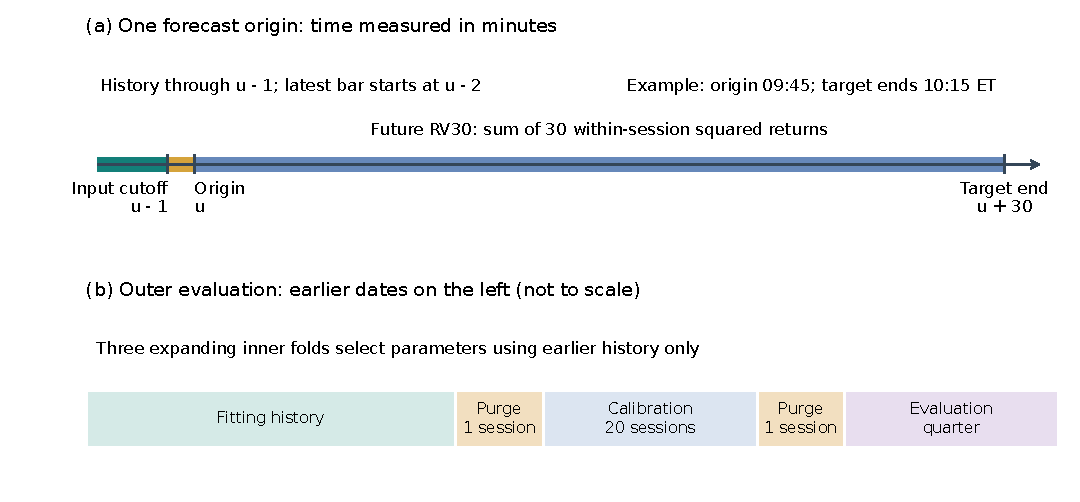
\includegraphics[width=0.98\textwidth]{images/task_and_validation.pdf}
\caption{Forecast timing and chronological evaluation. The upper panel shows the
one-minute input buffer and the subsequent 30-minute target. The lower
panel shows a fitting window, a separate 20-session calibration tail,
and one-session purge gaps before calibration and evaluation. Inner
selection uses three expanding temporal folds within the available outer
training history. The diagram represents the evaluation design, not
measured historical publication times.}
\label{fig:result-1}
\end{figure*}

\subsection{3.2. Coverage, inputs, and
eligibility}\label{coverage-inputs-and-eligibility}

We use Alpaca SIP historical minute OHLCV bars with raw adjustment from
4 January 2021 to 30 June 2026. The regular-session grid follows the New
York Stock Exchange calendar in \texttt{America/New\_York}, including
daylight-saving transitions and early closes. The retained period
contains 1,378 sessions and 535,620 expected bars per asset.

\begin{table}[!t]
\centering
\footnotesize
\caption{Historical regular-session bar coverage. AAPL is the only forecast target.}
\label{tab:results-1}
\begin{tabular}{lrrrl}
\toprule
Asset & Expected bars & Observed bars & Missing & Role \\
\midrule
AAPL & 535,620 & 535,620 & 0 & Target/input \\
SPY & 535,620 & 535,611 & 9 & Market input \\
QQQ & 535,620 & 535,620 & 0 & Market input \\
\bottomrule
\end{tabular}
\end{table}

The nine missing SPY bars remain missing. We reconstruct the retained
tables from the paginated raw responses and check the supplied fields
and selected unusual sessions. An overlapping subset of AAPL prices
received an additional source check; equivalent independent verification
is incomplete for SPY, QQQ, and volume. Historical final bars may
include revisions and do not identify their original arrival times.

The AAPL panel uses AAPL history. The market panel also supplies SPY and
QQQ history, with architecture-specific handling described below. Both
panels use common eligible evaluation origins, requiring the AAPL future
label and the historical inputs of all three assets. Future SPY and QQQ
labels do not determine evaluation eligibility. Auxiliary training
labels have separate eligibility checks. Long contexts and 22-session
aggregates impose additional history requirements. A retained historical
session can contain fewer than all scheduled origins; its mean loss uses
the eligible subset.

Development spans 2023Q1--2025Q2 and contains 602 eligible sessions and
207,235 origins per model. Historical confirmation spans 2025H2--2026H1
and contains 251 sessions and 86,306 origins. The earlier data supply
fitting history. These counts describe the evaluated sample after
eligibility rules, rather than the entire source calendar.

\section{4. Models and evaluation
protocol}\label{models-and-evaluation-protocol}

\subsection{4.1. Predictors and
representations}\label{predictors-and-representations}

The previous-RV reference uses the latest known 30-minute RV with a
fitting-window seasonal-ratio adjustment. HAR/HAR-X uses a prespecified
multiscale feature subset. Ridge and LightGBM search compact or richer
feature sets containing lagged 5-, 15-, 30-, 60-, and 120-minute
variation, previous-session and 5-/22-session aggregates, semivariances,
returns, historical volume/range measures, and trading-clock terms. All
features end at the same allowed cutoff. Scaling and seasonal profiles
use fitting observations only.

For Ridge, with transformed target \(z\) and standardized feature matrix
\(X\), we fit

\[
(\widehat b,\widehat\beta)
=\arg\min_{b,\beta}\{\|z-b-X\beta\|_2^2+\lambda\|\beta\|_2^2\},
\]

retaining an intercept and using an SVD solver. LightGBM searches tree
size, minimum leaf samples, learning rate, sampling, and regularization
under the fixed inner procedure. HAR is also tuned; it is not an
untreated default comparator.

Sequence models receive the history of trailing RV30 in log or log
seasonal-ratio form. The most recent known trailing value ends at
\(u-1\) minute. They predict 31 steps and use the last: the trailing
30-minute RV ending at \(u+30\) minutes equals the required future
target. Using the 30th step would produce a different window. Training
targets remain inside the permitted session and temporal partition.

xPatch retains the original architecture, with EMA/DEMA decomposition
options supported by the implementation. Its market panel learns
auxiliary asset tasks through shared channel-independent parameters; it
does not add a cross-channel fusion layer to the AAPL output. Tabular
models instead receive market features as conditional inputs. Chronos-2
uses a fixed checkpoint revision and file identities, and disables
cross-learning between separate forecast origins. Thus, the two panels
are not identical architectural ablations across families.

\subsection{4.2. Selection, calibration, and
confirmation}\label{selection-calibration-and-confirmation}

Each quarterly outer fold uses earlier dates for selection and fitting.
Before the outer quarter, we reserve a 20-session calibration tail, with
one whole-session purge gap on each side. Three expanding inner folds
contain non-overlapping 20-session validation blocks and apply the same
separation between fitting, calibration, and validation. We discard
labels crossing a partition boundary.

Training origins follow a fixed five-minute stride, inner validation a
ten-minute stride, and calibration and outer evaluation a one-minute
stride. These clock-based rules reduce duplicated work from overlapping
labels without selecting origins according to target values. Model
selection minimizes session-weighted inner QLIKE.

\begin{table}[!t]
\centering
\footnotesize
\caption{Registered search sizes per information set and outer fold. Configurations have model-specific computing costs.}
\label{tab:results-2}
\begin{tabular}{lp{.12\columnwidth}p{.42\columnwidth}}
\toprule
Model & Configs. & Inner selection \\
\midrule
Previous RV & 1 fixed & No search \\
HAR/HAR-X & 12 & Penalty, semivariances, representation \\
Ridge & 32 & Eight penalties, two feature sets, two representations \\
LightGBM & 80 & Fixed random search; inner early stopping \\
xPatch & 32 & Supported context, patch, decomposition, training settings \\
Chronos-2 & 8 & Four contexts, two representations; fixed weights \\
\bottomrule
\end{tabular}
\end{table}

LightGBM and xPatch screen configurations with seed 2026, then
reevaluate the top three using 2027 and 2028 on all three inner folds.
xPatch applies successive halving at cumulative epoch limits 5, 15, and
30, retaining 32, 16, and 8 configurations. Optimizer and random states
carry forward. Inner outcomes determine final training duration; outer
labels do not control early stopping. These are model-specific search
budgets with different computational costs.

For a positive raw variance forecast \(q_u\), the disjoint calibration
set \(\mathcal C\) supplies log residuals \(e_j=\log y_j-\log q_j\). We
obtain the point forecast and empirical interval endpoints from

\[
a=|\mathcal C|^{-1}\sum_{j\in\mathcal C}\exp(e_j),
\qquad \widehat y_u=a q_u,
\]

\[
\widehat I_u(\alpha)
=q_u[\exp(Q_{\alpha/2}(e)),\exp(Q_{1-\alpha/2}(e))].
\]

Here \(Q\) denotes an empirical quantile. For seasonal-ratio
predictions, \(q_u\) already includes the fitting-window seasonal
expectation at the future calendar positions. Calibration weights
eligible origins equally; evaluation weights sessions equally. These
empirical intervals have no distribution-free coverage guarantee.

Formal LightGBM and xPatch point forecasts average the three
individually calibrated variance means. Their ensemble intervals use
calibration log residuals around this arithmetic mean without altering
the point forecast. Deterministic models do not receive redundant seed
runs. The search record contains 100 tuned groups and 12,000 inner jobs,
or 120 groups and 12,200 jobs including fixed references and formal
outer prediction jobs. The supplement describes the retained ledger and
replay scope.

Only development-qualified candidates enter historical confirmation with
their corresponding HAR baselines. We retain the last development fold's
selected configuration, refit using only pre-confirmation data under the
same purge/calibration rules, and run no new search. This conditional
design cannot supply later-period rankings for models that were not
admitted.

\subsection{4.3. Loss, dependence, and joint
qualification}\label{loss-dependence-and-joint-qualification}

With a floor \(\varepsilon=10^{-12}\), let
\(\widetilde y=\max(y,\varepsilon)\) and
\(\widetilde p=\max(p,\varepsilon)\). The primary loss is

\[
L(y,p)=\frac{\widetilde y}{\widetilde p}
-\log\!\left(\frac{\widetilde y}{\widetilde p}\right)-1.
\]

For eligible origins \(\mathcal U_d\) in session \(d\), we compute

\[
\overline L_{m,d}=|\mathcal U_d|^{-1}
\sum_{u\in\mathcal U_d}L(y_u,\widehat y_{m,u}),
\]

then average \(\overline L_{m,d}\) equally across sessions. Early-close
sessions receive the same aggregate weight as full sessions. Relative
improvement is \(100(1-\overline L_m/\overline L_{HAR})\). Negative
values indicate higher loss than the matching HAR.

Paired daily differences are
\(D_{m,d}=\overline L_{m,d}-\overline L_{HAR,d}\). We use a one-sided
DM/HAC comparison with five session lags and Bartlett weights, plus
single-session and circular five-session bootstrap with 5,000 replicates
each. Uncentered bootstrap differences yield two-sided percentile
intervals; centered differences yield null tail probabilities. Blocks
follow observed eligible sessions without inserting artificial zero-loss
dates.

For each comparison, we take the maximum of the three p-values and apply
Holm adjustment to the fixed family of ten candidate/panel comparisons.
Qualification requires lower QLIKE, adjusted p below 0.05, negative
upper endpoints for both 95\% bootstrap intervals, improvement in at
least 7/10 quarters, improvement in each of 2023, 2024, and 2025H1, and
pooled/annual improvement for every prescribed seed. Confirmation
retains the corresponding statistical requirements, at least 3/4
improving quarters, and improvement in both half-year segments. These
additional stability requirements form a decision rule; they are not
separate proofs of uniform predictive superiority.

\subsection{4.4. Calibration diagnostics and study
status}\label{calibration-diagnostics-and-study-status}

We report log-RV MSE, empirical 80\%/90\% coverage and mean width with
equal session weights. We also fit the descriptive daily-mean regression

\[
\overline y_d=a_{MZ}+b_{MZ}\overline{\widehat y}_d+\epsilon_d,
\]

using HAC covariance with five session lags. Its daily observations
average overlapping intraday targets and forecasts. A slope near one
alone does not establish calibration: the intercept, uncertainty,
aggregation, and omitted conditional behavior also matter. We report
saved coefficient estimates and standard errors without introducing a
new joint hypothesis test.

The evaluation rules and configuration identities were signed locally
before the formal RV30 outer evaluation; this is not independent public
preregistration. The three RQs organize the present analysis after
results were known. Existing historical exposure and uncertain
checkpoint pretraining boundaries remain. Neither the narrative
organization nor numerical replay converts the study into an unexposed
test.

\section{5. Historical empirical
results}\label{historical-empirical-results}

\subsection{5.1. RQ1: Average loss and statistical
qualification}\label{rq1-average-loss-and-statistical-qualification}

Ridge achieves the lowest development QLIKE in both panels. Its
AAPL-only loss is 0.152919 against HAR's 0.165755, a 7.74\% improvement.
With market history, its loss is 0.152271 against 0.164462, a 7.41\%
improvement. Both comparisons have Holm p = 0.0019996 and satisfy the
joint qualification rule.

\begin{table*}[!t]
\centering
\footnotesize
\caption{Development results, 2023Q1--2025Q2. Gains are relative to the same-panel HAR; negative gains denote higher loss. All gates refers to the joint qualification rule.}
\label{tab:results-3}
\begin{tabular}{llrrrrl}
\toprule
Inputs & Model & QLIKE & Log-RV MSE & Gain (\%) & Holm p & All gates \\
\midrule
AAPL & Previous RV & 0.192281 & 0.345949 & −16.00 & 1 & Fail \\
AAPL & HAR & 0.165755 & 0.286719 & Reference & --- & Reference \\
AAPL & Ridge & 0.152919 & 0.257131 & 7.74 & 0.0019996 & Pass \\
AAPL & LightGBM & 0.156501 & 0.251059 & 5.58 & 0.0136551 & Fail \\
AAPL & xPatch & 0.160833 & 0.270772 & 2.97 & 0.330452 & Fail \\
AAPL & Chronos-2 & 0.177211 & 0.308747 & −6.91 & 1 & Fail \\
Market & Previous RV & 0.192281 & 0.345949 & −16.91 & 1 & Fail \\
Market & HAR-X & 0.164462 & 0.289572 & Reference & --- & Reference \\
Market & Ridge & 0.152271 & 0.257211 & 7.41 & 0.0019996 & Pass \\
Market & LightGBM & 0.158525 & 0.259838 & 3.61 & 0.330452 & Fail \\
Market & xPatch & 0.167298 & 0.276986 & −1.72 & 1 & Fail \\
Market & Chronos-2 & 0.178908 & 0.310045 & −8.78 & 1 & Fail \\
\bottomrule
\end{tabular}
\end{table*}

The five-session block intervals for Ridge minus HAR are {[}−0.017024,
−0.009415{]} and {[}−0.016843, −0.008327{]}. Figure 2 places these
paired effects alongside all other candidates. The intervals themselves
are pointwise; multiplicity enters through the separate Holm criterion.

\begin{figure*}[!t]
\centering
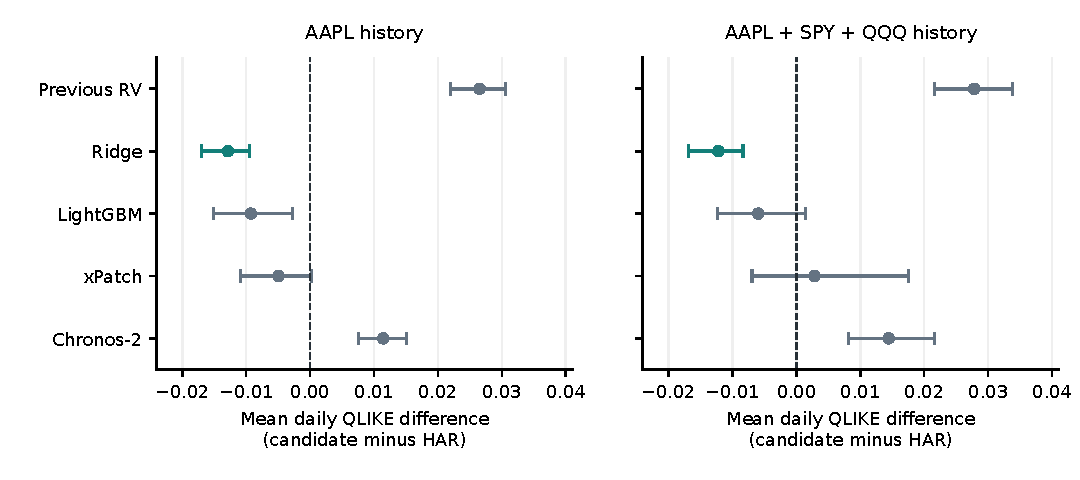
\includegraphics[width=0.98\textwidth]{images/development_loss_differences.pdf}
\caption{Mean daily QLIKE differences and pointwise 95\% five-session bootstrap
intervals. Negative differences favor the candidate over its matching
HAR. Green marks candidates satisfying all fixed qualification
requirements. The two panels use distinct HAR comparators; their
separate significance results do not test the difference between the two
Ridge forecasts.}
\label{fig:result-2}
\end{figure*}

AAPL-only xPatch improves mean QLIKE by 2.97\%, but its five-session
interval {[}−0.010903, 0.000159{]} includes zero and its adjusted p is
0.330452. Thus, a favorable mean alone does not establish improvement
under the protocol. Chronos-2 incurs higher QLIKE than HAR in both
panels. This finding applies to its fixed checkpoint, representation,
calibration, and eight searched configurations, rather than to
pretrained forecasting as a whole.

The market Ridge has slightly lower numerical QLIKE than AAPL-only
Ridge. The registered comparisons test each against its own HAR, so we
cannot attribute a statistically established incremental gain to SPY and
QQQ. The absence of a uniform market-panel benefit across families
further limits a simple interpretation of additional assets as
universally helpful inputs.

\subsection{5.2. RQ2: Temporal and seed
stability}\label{rq2-temporal-and-seed-stability}

The distinction between pooled performance and temporal stability is
most visible for LightGBM. In the AAPL panel it improves QLIKE by
5.58\%, has adjusted p = 0.013655, and has both bootstrap intervals
below zero. It also improves in 7/10 quarters. However, its improvement
turns negative in 2025H1, so it fails the annual-segment requirement.

\begin{table*}[!t]
\centering
\footnotesize
\caption{Annual-segment relative QLIKE improvements against the matching HAR. Better quarters counts negative daily-loss differences; the seed rule checks pooled and annual directions for the prescribed seeds.}
\label{tab:results-4}
\begin{tabular}{llrrrrl}
\toprule
Inputs & Model & 2023 (\%) & 2024 (\%) & 2025H1 (\%) & Quarters & Seed rule \\
\midrule
AAPL & Ridge & 4.48 & 8.93 & 10.57 & 10/10 & Pass \\
AAPL & LightGBM & 6.06 & 8.63 & −0.78 & 7/10 & Fail \\
AAPL & xPatch & 1.35 & 4.08 & 3.41 & 6/10 & Fail \\
AAPL & Chronos-2 & −4.52 & −7.60 & −9.32 & 1/10 & Fail \\
Market & Ridge & 2.32 & 10.17 & 9.56 & 9/10 & Pass \\
Market & LightGBM & −1.57 & 10.87 & −2.69 & 6/10 & Fail \\
Market & xPatch & −3.94 & 7.32 & −15.72 & 4/10 & Fail \\
Market & Chronos-2 & −13.92 & −4.65 & −9.20 & 1/10 & Fail \\
\bottomrule
\end{tabular}
\end{table*}

Each of the three LightGBM seeds has a positive 2025H1 loss difference
against HAR: 0.001292, 0.001798, and 0.001914. The deterioration
therefore appears across all prescribed seeds. These repeats measure
sensitivity to training randomness within one dataset; they do not
constitute independent market replications.

\begin{figure*}[!t]
\centering
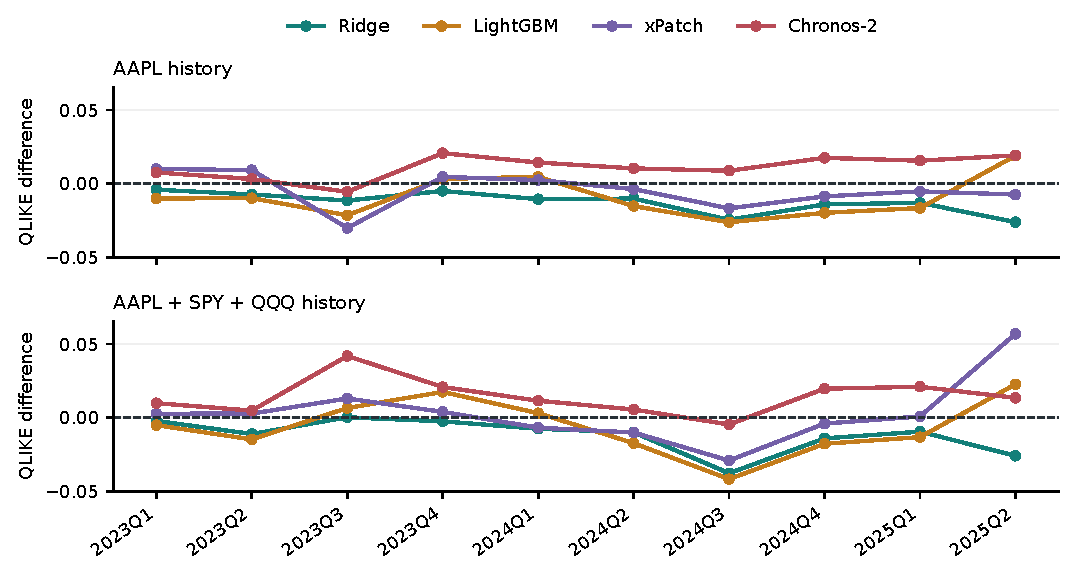
\includegraphics[width=0.98\textwidth]{images/quarterly_loss_differences.pdf}
\caption{Quarterly mean daily QLIKE differences relative to the matching HAR, for
all ten development quarters. Blue cells favor the candidate and red
cells favor HAR; values are descriptive differences. Both panels predict
AAPL. The display retains periods of deterioration and does not test
individual-quarter significance.}
\label{fig:result-3}
\end{figure*}

For AAPL-only xPatch, all three annual-segment ensemble means improve,
but only 6/10 quarters improve. Moreover, the 2027 and 2028 seed
predictions have positive 2023 differences of 0.000897 and 0.000673.
Annual aggregation and seed aggregation can therefore conceal different
failures. The market xPatch is more variable: its annual relative
changes are −3.94\%, +7.32\%, and −15.72\%.

Ridge improves in every AAPL-only quarter and nine market-panel
quarters, and in all three annual segments. Its deterministic fit has no
training-seed variability. These results support temporal consistency
within the evaluated periods; they do not guarantee improvement in every
future regime. The analysis locates instability but does not establish
whether distribution changes, estimation variance, input representation,
or another mechanism caused it.

\subsection{5.3. RQ3: Point losses and
calibration}\label{rq3-point-losses-and-calibration}

Model rankings depend on which forecast property is assessed. AAPL-only
LightGBM has lower log-RV MSE than Ridge, 0.251059 versus 0.257131,
while Ridge has lower QLIKE. Because the losses weight prediction errors
differently, we retain the prespecified variance-scale criterion instead
of selecting a metric after observing this reversal.

\begin{table*}[!t]
\centering
\footnotesize
\caption{Development empirical coverage and mean width. Widths are on the RV scale, multiplied by $10^5$; quantities use equal session weights.}
\label{tab:results-5}
\begin{tabular}{llrrrr}
\toprule
Inputs & Model & 80\% coverage & 80\% width & 90\% coverage & 90\% width \\
\midrule
AAPL & Previous RV & 78.79\% & 1.5071 & 89.31\% & 2.1601 \\
AAPL & HAR & 79.12\% & 1.1610 & 88.83\% & 1.6126 \\
AAPL & Ridge & 79.33\% & 1.4147 & 88.88\% & 1.9232 \\
AAPL & LightGBM & 79.40\% & 0.9966 & 88.90\% & 1.3708 \\
AAPL & xPatch & 80.16\% & 1.1575 & 89.59\% & 1.5940 \\
AAPL & Chronos-2 & 79.63\% & 1.2958 & 89.57\% & 1.8322 \\
Market & Previous RV & 78.79\% & 1.5071 & 89.31\% & 2.1601 \\
Market & HAR-X & 78.89\% & 1.1492 & 88.70\% & 1.5827 \\
Market & Ridge & 78.66\% & 1.2913 & 88.59\% & 1.7851 \\
Market & LightGBM & 78.05\% & 0.9894 & 88.01\% & 1.3691 \\
Market & xPatch & 80.37\% & 1.0791 & 89.45\% & 1.4880 \\
Market & Chronos-2 & 79.43\% & 1.3144 & 89.46\% & 1.8565 \\
\bottomrule
\end{tabular}
\end{table*}

Widths in Table 5 are multiplied by \(10^5\). Ridge's development
intervals are wider than the corresponding HAR intervals, while
AAPL-only xPatch has aggregate coverage closer to nominal and narrower
intervals than Ridge. These observations address different objects from
the mean-forecast QLIKE comparison. No uncertainty-adjusted
interval-quality ranking was specified or established.

Period-specific results expose a limitation hidden by aggregate
coverage. AAPL-only Ridge's 90\% coverage is 88.76\% in 2023, 90.48\% in
2024, and 85.82\% in 2025H1. During 2025H1, its QLIKE improves by
10.57\%, while average 90\% width is 4.7908 on the displayed scale,
against HAR's 2.8996. Lower point loss thus coexists with under-coverage
and greater width in that segment. HAR and xPatch also under-cover
there, at 86.18\% and 86.99\%. The observations motivate local
uncertainty diagnostics without identifying a particular source of
miscalibration.

The daily-mean regression provides a further view. Development slopes
for Ridge are 0.370 and 0.482, with positive intercepts; their later
confirmation slopes are near one. Table 6 reports the coefficient
estimates and saved HAC slope standard errors.

\begin{table*}[!t]
\centering
\footnotesize
\caption{Daily-mean observed-on-predicted regression. Intercepts use RV units multiplied by $10^5$. Slope standard errors use the saved five-lag HAC covariance; no new joint calibration test is performed.}
\label{tab:results-6}
\begin{tabular}{lllrrr}
\toprule
Period & Inputs & Model & Intercept $\times10^5$ & Slope & HAC SE \\
\midrule
Development & AAPL & HAR & −0.6158 & 1.616 & 0.191 \\
Development & AAPL & Ridge & 0.5850 & 0.370 & 0.025 \\
Development & Market & HAR-X & −0.6546 & 1.639 & 0.190 \\
Development & Market & Ridge & 0.4720 & 0.482 & 0.024 \\
Confirmation & AAPL & HAR & −0.2702 & 1.148 & 0.069 \\
Confirmation & AAPL & Ridge & −0.1431 & 1.049 & 0.057 \\
Confirmation & Market & HAR-X & −0.1867 & 1.037 & 0.054 \\
Confirmation & Market & Ridge & −0.1619 & 1.053 & 0.057 \\
\bottomrule
\end{tabular}
\end{table*}

A slope below one in this observed-on-predicted regression describes its
fitted relation; it does not by itself imply compressed forecast
variance. Development pools quarterly refits, whereas confirmation uses
one pre-period refit, so coefficient changes cannot be attributed solely
to a change in calibration quality. We neither test a new joint
intercept/slope hypothesis nor infer conditional or prospective
calibration from these summaries.

\subsection{5.4. Subsequent historical
confirmation}\label{subsequent-historical-confirmation}

Both qualified Ridge candidates retain lower QLIKE in the 251-session
confirmation sample. They improve in all four quarters and pass the
fixed confirmation requirements. The AAPL-only reduction is 6.29\%; the
market-panel reduction is 7.97\%.

\begin{table*}[!t]
\centering
\footnotesize
\caption{Historical confirmation, 2025H2--2026H1. Intervals are five-session block intervals for Ridge minus HAR.}
\label{tab:results-7}
\begin{tabular}{lrrrrl}
\toprule
Inputs & HAR QLIKE & Ridge QLIKE & Gain (\%) & Holm p & Five-session 95\% CI \\
\midrule
AAPL & 0.175851 & 0.164782 & 6.29 & 0.0019996 & {[}−0.013920, −0.008246{]} \\
Market & 0.174630 & 0.160710 & 7.97 & 0.0019996 & {[}−0.017701, −0.009876{]} \\
\bottomrule
\end{tabular}
\end{table*}

AAPL-only Ridge's 80\%/90\% coverage is 81.63\%/90.90\%, with mean
widths 1.0291/1.4839 on the displayed scale. Market Ridge has
81.52\%/90.56\% coverage and widths 1.0471/1.4768. These remain
descriptive historical diagnostics. Since only development-qualified
candidates entered this stage, the results establish no
confirmation-period superiority over the excluded model families. The
previously exposed confirmation dates supply later-period consistency
evidence with a fixed configuration, rather than independent blind or
live validation.

\section{6. Discussion}\label{discussion}

The three research questions lead to distinct conclusions. Ridge meets
the aggregate and stability requirements in both panels. LightGBM's
AAPL-only aggregate improvement fails the temporal requirements, and
xPatch's favorable ensemble mean fails the joint statistical rule.
Meanwhile, calibration diagnostics qualify the interpretation of Ridge's
point-loss advantage. A model can be the preferred mean predictor under
the fixed QLIKE rule without supplying sufficiently reliable intervals
in each period.

Ridge's performance is consistent with the usefulness of regularization
when engineered features already summarize persistence and the trading
clock. This is an interpretation to test, not a demonstrated mechanism.
The study does not isolate the effects of regularization, feature
design, training sample size, or the choice of representation. A
comparison of the same architecture with and without each component, on
separately protected evaluation data, would be needed to support those
attributions.

The stability rule changes the decision made from pooled significance.
It rejects AAPL-only LightGBM despite its adjusted p below 0.05 because
its 2025H1 deterioration conflicts with a stated requirement. That
requirement embodies a preference for consistency across the selected
segments. Different applications could justify other tolerances, but
changing them after seeing these results would define a new selection
problem. We retain the original rule and report the conflicting
diagnostics.

The calibration findings also discourage collapsing uncertainty
assessment into point-score selection. Empirical residual quantiles can
deliver near-nominal aggregate coverage while missing within particular
periods. Daily-mean regression discards intraday conditional structure,
and average width alone does not quantify the cost of all coverage
errors. Accordingly, these diagnostics identify limitations in the
evaluated uncertainty outputs; they do not establish a uniformly
superior probabilistic forecasting method.

\section{7. Limitations and future
work}\label{limitations-and-future-work}

\textbf{Generalization and comparability.} We evaluate one target asset
and one horizon. SPY and QQQ history extends inputs or auxiliary
training, not the number of independently evaluated targets. Model
families differ in feature access, input representation, and search
costs. The market panel has different structural effects on tabular
models and channel-independent xPatch. A useful next study would
evaluate AAPL, SPY, and QQQ as separate targets under explicitly matched
available information, with chronological selection and a fixed
comparison family. Because these assets are correlated, even that
extension would not establish broad cross-market generalization.

\textbf{Historical and statistical boundaries.} Previously exposed
dates, incomplete historical-arrival records, possible data revisions,
and uncertain pretraining contamination limit interpretation. One-minute
RV is an imperfect proxy, and calendar completeness does not ensure the
absence of data defects. Daily aggregation addresses much of the
intraday overlap but does not create independent sessions or eliminate
all forms of nonstationarity. Bootstrap and HAC results depend on the
fixed resampling and lag choices. Two local replay rounds check
computation and saved artifacts; they are not independent-provider or
external-laboratory replication.

\textbf{Controlled simulation.} A prospective supplement could test
stable GARCH dynamics, predetermined variance shifts, and leverage or
heavy-tailed innovations while retaining known generation rules. Matched
innovation draws, independent generated paths, and locked
development/test boundaries would allow analysis of whether average
losses hide local deterioration. The simulation should report interval
width alongside coverage and define recovery criteria before observing
results. No such simulation results are included in the present study.
Simulation would test behavior under the chosen processes; it would not
establish the cause of the historical AAPL ranking or replace market
validation.

\textbf{Timely prospective and economic validation.} The frozen models
require evaluation on genuinely later, timely received data with actual
issue timestamps. Free delayed SIP can support a separate shadow replay
of the same market-time task, but generation after the origin cannot
establish a forecast issued before its target window. Timely evaluation
should preserve model identities and assess a fixed sample without
interim score-based updates. Directional trading returns, transaction
costs, spreads, slippage, and execution rules have not been evaluated.
Historical variance-loss reductions cannot be converted into
profitability claims. These are future empirical studies rather than
missing values to infer from the current results.

\section{8. Conclusion}\label{conclusion}

For the evaluated AAPL RV30 task, tuned Ridge improves QLIKE over its
corresponding HAR and meets the fixed stability requirements in
development and later historical confirmation. AAPL-only LightGBM
demonstrates that pooled statistical improvement can coexist with a
failed temporal requirement. Calibration diagnostics show that even the
preferred point predictor can under-cover an annual segment. The
practical implication within this setting is to retain strong
regularized baselines and assess average error, temporal stability, and
uncertainty separately. The evidence remains historical and
task-specific; matched-input, multi-target, simulated-mechanism, and
timely prospective studies are needed for broader conclusions.

\section{Data and code availability}\label{data-and-code-availability}

The local reproducibility package indexes the protocol, configurations,
data and checkpoint identities, predictions, search ledger, and
verification scope through \texttt{delivery/manifest.json}. The
accompanying supplementary material describes table and figure
reproduction and provides saved annual, seed, clock, and calibration
diagnostics. Historical source bars require appropriate Alpaca access;
redistribution rights are not established here. The project repository
is https://github.com/wyyyyy-0121/xPatch, but this manuscript does not
assert that its complete current local results and artifacts have been
published there. The availability of a complete public replication
package remains to be established before submission.

\section*{References}
\begingroup\small

{[}1{]} Andersen, T. G., Bollerslev, T., Diebold, F. X., and Labys, P.
(2003). Modeling and Forecasting Realized Volatility.
\emph{Econometrica}, 71(2), 579--625.
https://doi.org/10.1111/1468-0262.00418.

{[}2{]} Corsi, F. (2009). A Simple Approximate Long-Memory Model of
Realized Volatility. \emph{Journal of Financial Econometrics}, 7(2),
174--196. https://doi.org/10.1093/jjfinec/nbp001.

{[}3{]} Andersen, T. G., and Bollerslev, T. (1997). Intraday periodicity
and volatility persistence in financial markets. \emph{Journal of
Empirical Finance}, 4(2--3), 115--158.
https://doi.org/10.1016/S0927-5398(97)00004-2.

{[}4{]} Patton, A. J. (2011). Volatility forecast comparison using
imperfect volatility proxies. \emph{Journal of Econometrics}, 160(1),
246--256. https://doi.org/10.1016/j.jeconom.2010.03.034.

{[}5{]} Patton, A. J., and Sheppard, K. (2015). Good Volatility, Bad
Volatility: Signed Jumps and the Persistence of Volatility. \emph{Review
of Economics and Statistics}, 97(3), 683--697.
https://doi.org/10.1162/REST\_a\_00503.

{[}6{]} Diebold, F. X., and Mariano, R. S. (1995). Comparing Predictive
Accuracy. \emph{Journal of Business \& Economic Statistics}, 13(3),
253--263. https://doi.org/10.1080/07350015.1995.10524599.

{[}7{]} Stitsyuk, A., and Choi, J. (2025). xPatch: Dual-Stream Time
Series Forecasting with Exponential Seasonal-Trend Decomposition.
\emph{Proceedings of the AAAI Conference on Artificial Intelligence},
39(19), 20601--20609. https://doi.org/10.1609/aaai.v39i19.34270.

{[}8{]} Ansari, A. F., Shchur, O., Küken, J., et al.~(2025). Chronos-2:
From Univariate to Universal Forecasting. arXiv:2510.15821.
https://arxiv.org/abs/2510.15821.

{[}9{]} Hoerl, A. E., and Kennard, R. W. (1970). Ridge Regression:
Biased Estimation for Nonorthogonal Problems. \emph{Technometrics},
12(1), 55--67. https://doi.org/10.1080/00401706.1970.10488634.

{[}10{]} Ke, G., Meng, Q., Finley, T., et al.~(2017). LightGBM: A Highly
Efficient Gradient Boosting Decision Tree. \emph{Advances in Neural
Information Processing Systems}, 30.
https://www.microsoft.com/en-us/research/wp-content/uploads/2017/11/lightgbm.pdf.

{[}11{]} Newey, W. K., and West, K. D. (1987). A Simple, Positive
Semi-Definite, Heteroskedasticity and Autocorrelation Consistent
Covariance Matrix. \emph{Econometrica}, 55(3), 703--708.
https://doi.org/10.2307/1913610.

{[}12{]} Holm, S. (1979). A Simple Sequentially Rejective Multiple Test
Procedure. \emph{Scandinavian Journal of Statistics}, 6(2), 65--70.
https://www.jstor.org/stable/4615733.

{[}13{]} Gijsbers, P., Bueno, M. L. P., Coors, S., LeDell, E., Poirier,
S., Thomas, J., Bischl, B., and Vanschoren, J. (2024). AMLB: an AutoML
Benchmark. \emph{Journal of Machine Learning Research}, 25(101), 1--65.
https://www.jmlr.org/papers/v25/22-0493.html.

{[}14{]} Pacchiardi, L., Adewoyin, R. A., Dueben, P., and Dutta, R.
(2024). Probabilistic Forecasting with Generative Networks via Scoring
Rule Minimization. \emph{Journal of Machine Learning Research}, 25(45),
1--64. https://www.jmlr.org/papers/v25/23-0038.html.

{[}15{]} Gibbs, I., and Candès, E. J. (2024). Conformal Inference for
Online Prediction with Arbitrary Distribution Shifts. \emph{Journal of
Machine Learning Research}, 25(162), 1--36.
https://www.jmlr.org/papers/v25/22-1218.html.

\endgroup

\end{document}
